\documentclass[a4paper,12pt]{article}

% Character set
\usepackage{cmap}
\usepackage[utf8]{inputenc}
\usepackage[T1]{fontenc} % ensure that all the characters in characterSets.tex prints
\usepackage{upquote} % \textcent
\usepackage{pifont} % add \ding, http://ctan.org/pkg/pifont

% A background text to prevent wide distribution
\usepackage{draftwatermark}
\SetWatermarkText{DRAFT}
\SetWatermarkScale{6}
\SetWatermarkLightness{.95}

% Page setup
\usepackage[top=25mm,bottom=20mm,inner=20mm,outer=40mm,marginparsep=3mm,marginparwidth=35mm]{geometry}
\renewcommand{\floatpagefraction}{.8}%

% paragraph indentation is stupid
\setlength\parindent{0pt}
\setlength{\parskip}{1em}

% Globally defined colors
\usepackage[table,x11names]{xcolor}
\definecolor{alternateKeywordsColor}{rgb}{0.13,1,0.13}
\definecolor{keywordsColor}{rgb}{0.13,0.13,1}
%\definecolor{commentsColor}{rgb}{0,0.5,0}
\definecolor{commentsColor}{rgb}{0,0.5,0}
%\definecolor{stringsColor}{rgb}{0.9,0,0}
\definecolor{stringsColor}{rgb}{0,0,0.5}
\definecolor{light-gray}{gray}{0.95}
\definecolor{codeLineHighlight}{named}{SlateGray1}
%\definecolor{codeLineHighlight}{rgb}{0.975,0.975,0.975}
\definecolor{syntaxColor}{rgb}{0,.45,0}

\definecolor{headerRowColor}{rgb}{0.85,0.85,0.85}
\definecolor{oddRowColor}{rgb}{0.95,0.95,0.95}
\definecolor{evenRowColor}{rgb}{1,1,1}

% add check- and crossmarks, http://ctan.org/pkg/pifont
\newcommand{\cmark}{{\color{green}\ding{51}}}%
\newcommand{\xmark}{{\color{red}\ding{55}}}%

% Extra math stuff
\usepackage{amsmath,amssymb}

% Typeset chess
\usepackage{skak}

% Figures
\usepackage{graphicx}
\graphicspath{{figures/}}

% clickable url
\usepackage{url}

% figures
\usepackage{subfigure}

% Clickable table of content
\usepackage[pdfpagelabels]{hyperref}
%\usepackage{multirow}
\usepackage{makecell}

% Include label name in ref
\usepackage[noabbrev,capitalize]{cleveref}
\newcommand{\creflastconjunction}{, and\nobreakspace~}
\Crefformat{tcb@cnt@codeNOutput}{Listing~#2#1#3}
\crefformat{tcb@cnt@codeNOutput}{Listing~#2#1#3}
\crefrangeformat{tcb@cnt@codeNOutput}{Listing~#3#1#4\nobreakdash--#5#2#6}
\Crefrangeformat{tcb@cnt@codeNOutput}{Listing~#3#1#4\nobreakdash--#5#2#6}
\crefmultiformat{tcb@cnt@codeNOutput}{Listing~#2#1#3}{ and~#2#1#3}{, #2#1#3}{\creflastconjunction#2#1#3}
\Crefmultiformat{tcb@cnt@codeNOutput}{Listing~#2#1#3}{ and~#2#1#3}{, #2#1#3}{\creflastconjunction#2#1#3}
\crefrangeformat{table}{Table~#3#1#4\nobreakdash--#5#2#6}
\Crefrangeformat{table}{Table~#3#1#4\nobreakdash--#5#2#6}
\crefrangeformat{part}{Part~#3#1#4\nobreakdash--#5#2#6}
\Crefrangeformat{part}{Part~#3#1#4\nobreakdash--#5#2#6}

% paragraphs in tables
\usepackage{tabularx}

% formatting lists
\usepackage{enumitem}
%\setlist[description]{leftmargin=0pt,labelindent=0pt,itemindent=0pt}
%\setlist[description]{itemindent=-\leftmargin}

% latex comment environment
\usepackage{comment}

% UML
\usepackage{pgf-umlcd}
\renewcommand{\umltextcolor}{black} 
\renewcommand{\umlfillcolor}{black!5!white}
\renewcommand{\umldrawcolor}{teal}

% List of indices
\usepackage{xstring}
\usepackage{makeidx}
\usepackage{marginfix} % fixes marginpar location problem in 2 -page mode.
\newcommand{\idxs}[1]{\marginpar{$\cdot$~\parbox[t]{\linewidth}{\raggedright \expandarg\IfSubStr{#1}{@}{\StrBehind{#1}{@}}{#1}}}\index{#1}} % The parbox is too wide, since the line also includes cdot-space
\newcommand{\idxss}[1]{\index{#1}}
% Define a new command idx with an optional parameter, which if given is the key to the index
\makeatletter
\def\idx{\@ifnextchar[{\@with}{\@without}}
\def\@with[#1]#2{\emph{#2}\idxs{#1}}
\def\@without#1{\emph{#1}\idxs{#1}}
\makeatother
%\newcommand{\idx}[1]{\emph{#1}\idxs{#1}}
\newcommand{\keyword}[1]{{\lstinline[language=fsharp]|#1|}}
\newcommand{\lexeme}[1]{\mbox{``\lstinline[language=fsharp]|#1|''}}
\makeindex

% display tree like structures
\usepackage{qtree}

% We frame all listings and problems
\usepackage{tcolorbox}
\tcbuselibrary{listings}
\tcbuselibrary{raster}
\tcbset{%
  colframe=teal, %PaleGreen1!45!black,
  %coltitle=black,
  fonttitle=\bfseries, 
  leftrule=3mm,
  sharp corners=downhill,
  colback=black!5!white,
  left=1mm,
  top=1mm,
  right=1mm,
  bottom=1mm,
  middle=1mm,
  arc=2mm,
}
\newtcolorbox[auto counter]{problem}[1][]{%
  title=\textbf{Problem~\thetcbcounter},
  colframe=DeepSkyBlue1, %green!30!blue,
  #1}
\newcommand{\src}{src}
\newtcolorbox[auto counter]{codeNOutput}[2][]{%
  title=\textbf{Listing~\thetcbcounter#2},
  #1}

%% lstlisting stuff
\usepackage{listings} 
\def\lstfs#1{\mbox{\lstinline{{#1}}}}
% Get counters from references for firstnumber references in lstinputlisting
\usepackage{refcount}
\newcounter{lstFrom}
\newcounter{lstTo}
% Example: 
% \setcounterref{lstFrom}{dynamicScopeTracing:a1}
% \setcounterref{lstTo}{dynamicScopeTracing:a2}
% \lstinputlisting[firstline=\thelstFrom,lastline=\thelstTo,escapechar=|]{\src/dynamicScopeTracing.fsx}
\usepackage{lstlinebgrd}
\makeatletter
%The following sets the box compatible with tcolorbox setup
\def\lst@linebgrdcolor{\color{black!5!white}}
\def\lst@linebgrdsep{1em}
\def\lst@linebackgroundwidth{1em}
\def\lst@linebackgroundhighlight{\color{codeLineHighlight}}
\renewcommand{\lst@linebgrd}{%
  \ifx\lst@linebgrdcolor\empty
  \else
    \rlap{
       \lst@basicstyle\color{black!5!white} % tcolorbox background color
       \lst@linebgrdcolor{
          \kern-\dimexpr\lst@linebgrdsep\relax
          \lst@linebgrdcmd{\lst@linebgrdwidth}{\lst@linebgrdheight}{\lst@linebgrddepth}
       }
    }
  \fi
}
% Highlight a range of lines with green. Use \getrefnumber{label} for refs
\newcommand{\highlightRange}[2]{\ifnum\value{lstnumber}>\numexpr#1-1\ifnum\value{lstnumber}<\numexpr1+#2\lst@linebackgroundhighlight\fi\fi}
% \highlight conflicts with skak. Just rewriting, wonder what breaks in skak
\renewcommand{\highlight}[1]{\ifnum\value{lstnumber}=#1\lst@linebackgroundhighlight\fi}

% To use verbatimwrite to write listing to file, e.g., in conjunction with ebnfs
\usepackage{moreverb} 

\lstdefinelanguage{fsharp}{%
  keywords={abstract, and, as, assert, base, begin, class, default, delegate, do, done, downcast, downto, elif, else, end, exception, extern, false, finally, for, fun, function, global, if, in, inherit, inline, interface, internal, lazy, let, match, member, module, mutable, namespace, new, null, of, open, or, override, private, public, rec, return, sig, static, struct, then, to, true, try, type, upcast, use, val, void, when, while, with, yield},
  morekeywords={atomic, break, checked, component, const, constraint, constructor, continue, eager, fixed, fori, functor, include, measure, method, mixin, object, parallel, params, process, protected, pure, recursive, sealed, tailcall, trait, virtual, volatile},
  otherkeywords={ let!, return!, do!, yield!, use!},
  keywordstyle=\color{keywordsColor},
  % sensitive=true,
  basicstyle=\ttfamily\lst@ifdisplaystyle\small\fi, % make font small for listings but not for lstinline
  breaklines=true,
  breakatwhitespace=true
  showstringspaces=false,
  morecomment=[l][\color{commentsColor}]{///},
  morecomment=[l][\color{commentsColor}]{//},
  morecomment=[n][\color{commentsColor}]{(*}{*)},
  morecomment=[is][\color{white}]{(*//}{*)},
  morestring=[b]",
  literate={`}{\`}1,
  stringstyle=\color{stringsColor},
  showspaces=true,
  numbers=left,
  numbersep=6pt,
  numberstyle=\scriptsize\color{white},
  % aboveskip=0pt, 
  % belowskip=0pt,
  % resetmargins=true,
  % captionpos=b,
  backgroundcolor=\color{black!5!white},
}


\lstdefinelanguage{syntax}{%
  classoffset=0,
  keywords={abstract, and, as, assert, base, begin, class, default, delegate, do, done, downcast, downto, elif, else, end, exception, extern, false, finally, for, fun, function, global, if, in, inherit, inline, interface, internal, lazy, let, match, member, module, mutable, namespace, new, null, of, open, or, override, private, public, rec, return, sig, static, struct, then, to, true, try, type, upcast, use, val, void, when, while, with, yield, atomic, break, checked, component, const, constraint, constructor, continue, eager, fixed, fori, functor, include, measure, method, mixin, object, parallel, params, process, protected, pure, recursive, sealed, tailcall, trait, virtual, volatile, let!, return!, do!, yield!, use!},
  keywordstyle=\color{keywordsColor},
  % classoffset=1,
  % morekeywords={ident, expr, arg, format-string},
  % keywordstyle=\color{syntaxColor},
  % classoffset=0,
  otherkeywords={},
  basicstyle=\ttfamily\lst@ifdisplaystyle\small\fi, % make font small for listings but not for lstinline
  breaklines=true,
  breakatwhitespace=true
  showstringspaces=false,
  classoffset=0,
  morecomment=[l][\color{commentsColor}]{////},
  literate={`}{\`}1 {\{*}{{{\color{syntaxColor}\{}}}1 {*\}}{{{\color{syntaxColor}\}}}}1 {[*}{{{\color{syntaxColor}[}}}1  {*]}{{{\color{syntaxColor}]}}}1 {|*}{{{\color{syntaxColor}|}}}1, % {etc*}{{{\color{syntaxColor}...}}}3,
  moredelim  = **[is][\processmydelims]{<*}{*>}, % delete delimiters, typeset keywords. Don't know how to avoid the last...
  showspaces=true,
  numbers=left,
  numbersep=6pt,
  numberstyle=\scriptsize\color{white},
  backgroundcolor=\color{black!5!white},
}
%Tweek of deliminter and literate: https://tex.stackexchange.com/questions/203263/listings-package-custom-language-delimiter-match-left-side
\newcommand\processmydelimsend{}
\newcommand\processmydelims{%
  \renewcommand\processmydelimsend{\textcolor{syntaxColor}{>}\egroup}%
  \bgroup\color{syntaxColor}<\aftergroup\processmydelimsend%
}
% \makeatletter
% \newcommand\processhash{%
%   \ifnum\lst@mode=\lst@Pmode%
%     \bfseries%
%   \fi
%   \#%
% }
% \makeatother


\lstdefinelanguage{ebnf}{%
  keywords={},
  morekeywords={},
  otherkeywords={},
  keywordstyle=\color{keywordsColor},
  % sensitive=true,
  basicstyle=\fontfamily{pcr}\selectfont\lst@ifdisplaystyle\small\fi, 
  breaklines=true,
  breakatwhitespace=true
  morecomment=[s][\color{commentsColor}]{(*}{*)},
  morestring=[b]",
  morestring=[b]',
  alsoletter={\\},
  showstringspaces=false,
  % stringstyle=\color{stringsColor},
  % aboveskip=0pt, 
  % belowskip=0pt,
  % resetmargins=true,
  % captionpos=b,
  % backgroundcolor=\color{blue!10!white},
}
\lstdefinelanguage{console}{%
  keywords={},
  morekeywords={},
  otherkeywords={},
  basicstyle=\ttfamily\lst@ifdisplaystyle\small\fi, 
  breaklines=true,
  showstringspaces=false,
  % aboveskip=0pt,
  % belowskip=0pt,
  % resetmargins=true,
  % captionpos=b,
  % backgroundcolor=\color{green!10!white},
}
%\lstset{language=fsharp, frame=single}
\lstset{language=fsharp,showlines=false}
\makeatletter
\def\lst@visiblespace{ }
\makeatother

% input .fsx and .out listings from \src and display as code and result in same figure
% #1 = optional further arguments for lstinputlisting
% #2 = filename without suffix, and label
% #3 = caption
\newtcbinputlisting[use counter from=codeNOutput]{\fs}[3][]{%
  listing file={src/#2.fsx},
  listing and comment,
  listing options={language=fsharp,escapechar=§,#1},
  title=\textbf{Listing \thetcbcounter} {#2.fsx:\\#3},
  label={#2},
  comment={\lstinputlisting[language=console]{\src/#2.out}}
}

% dispaly fsharp code \src
% #1 = optional further arguments for lstinputlisting
% #2 = filename
% #3 = label
% #4 = caption
\newtcbinputlisting[use counter from=codeNOutput]{\fsharp}[4][]{%
  listing file={\src/#2},
  listing only,
  listing options={language=fsharp,escapechar=§,#1},
  title=\textbf{Listing \thetcbcounter} {#2:\\#4},
  label={#3},
}

% dispaly console file \src
% #1 = optional further arguments for lstinputlisting
% #2 = filename
% #3 = label
% #4 = caption
\newtcbinputlisting[use counter from=codeNOutput]{\console}[4][]{%
  listing file={\src/#2},
  listing only,
  listing options={language=console,escapechar=§,#1},
  title=\textbf{Listing \thetcbcounter} {#2:\\#4},
  label={#3},
}

\newtcbinputlisting[use counter from=codeNOutput]{\fsCode}[4]{%
  listing file={src/#1.fsx},
  listing only,
  listing options={language=fsharp,escapechar=§,#4},
  title=\textbf{Listing \thetcbcounter} {#1.fsx:\\#3},
  label={#2},
}

% dispaly ebnf file, no label
% #1 = optional further arguments for lstinputlisting
% #2 = filename
% #3 = caption
\newtcbinputlisting[use counter from=codeNOutput]{\ebnf}[3][]{%
  listing file={#2},
  listing only,
  colframe=black!50!white,
  listing options={language=ebnf,escapechar=§,#1},
  title=\textbf{Listing \thetcbcounter} {#3},
}

% dispaly syntax file, no label
% #1 = optional further arguments for lstinputlisting
% #2 = filename without suffix, and label
% #3 = caption
\newtcbinputlisting[use counter from=codeNOutput]{\syntax}[3][]{%
  listing file={#2},
  listing only,
  colframe=black!50!white,
  listing options={language=syntax,escapechar=§,#1},
  title=\textbf{Listing \thetcbcounter} {#3},
  label={#2}
}

\newtcbinputlisting[use counter from=codeNOutput]{\fsSignature}[4]{%
  listing file={src/#1.fsi},
  listing only,
  listing options={language=fsharp,escapechar=§,#4},
  title=\textbf{Listing \thetcbcounter} {#1.fsi:\\#3},
  label={#2},
}
\newtcbinputlisting[use counter from=codeNOutput]{\fsImplementation}[4]{%
  listing file={src/#1.fs},
  listing only,
  listing options={language=fsharp,escapechar=§,#4},
  title=\textbf{Listing \thetcbcounter} {#1.fs:\\#3},
  label={#2},
}

% dispaly output file .out from \src
% #1 = optional further arguments for lstinputlisting
% #2 = filename without suffix, and label
% #3 = caption
\newtcbinputlisting[use counter from=codeNOutput]{\fsOutput}[3][]{%
  listing file={src/#2.out},
  listing only,
  listing options={language=console,escapechar=§,#1},
  title=\textbf{Listing \thetcbcounter}: {#3},
  label={#2},
}

% dispaly output file .out from \src as an element in tabularx
% #1 = optional further arguments for lstinputlisting
% #2 = filename without suffix, and label
% #3 = caption
\newtcbinputlisting[use counter from=codeNOutput]{\fsOutputTabx}[3][]{%
  listing file={src/#2.out},
  listing only,
  width=\hsize,
  box align=top,
  listing options={language=console,escapechar=§,aboveskip=0pt,belowskip=0pt,emptylines=0,#1},
  title=\textbf{Listing \thetcbcounter}: {#3},
  label={#2},
}

\newcommand{\filename}[1]{\lstinline[language=console]{#1}}

% highlighted text snippets
\newcommand{\advice}[1]{\marginpar{Advice}{\textbf{#1}}}
\newcommand{\advanced}[1]{\marginpar{Advanced material}\textbf{#1}}

% sometimes we need to include hash sign as arguments
\begingroup\catcode`\#=12
\newcommand\hashchar{}%check that is doesn't exist
\gdef\hashchar{#}
\endgroup

% Scratch out math, used in test.tex
\usepackage{cancel}
%\newcommand{\bcancel}[1]{#1}

% Draw arrows between elements
\usepackage{tikz}
%\usepackage{sphack} % make overlays invisible where stated in text
\usetikzlibrary{arrows,shapes,calc,decorations.pathreplacing}
\newcommand{\tikzmark}[1]{\tikz[overlay,remember picture] \node (#1) {};}
\newcommand*{\DrawArrow}[3][]{%
  % #1 = draw options
  % #2 = left point
  % #3 = right point
  \begin{tikzpicture}[overlay,remember picture]
    %\draw [-latex, #1,ultra thick,red] ($(#2)+(0.1em,0.5ex)$) to ($(#3)+(0,0.5ex)$);
    \draw [-latex, #1,ultra thick,red] ($(#2) -(0,0.5ex)$) to ($(#3)+(0,2ex)$);
  \end{tikzpicture}%
}%
\newcommand*{\AddNote}[4]{%
  \begin{tikzpicture}[overlay, remember picture]
    \draw [decoration={brace,amplitude=0.5em},decorate,ultra thick,red]
    ($(#3)!([yshift=1.5ex]#1)!($(#3)-(0,1)$)$) -- ($(#3)!(#2)!($(#3)-(0,1)$)$)
    node [align=left, text width=0cm, pos=0.5, anchor=west, xshift=.2cm] {#4};
  \end{tikzpicture}
}%
\newcommand{\FrameArea}[2]{%
  % #1 = top left point
  % #2 = bottom right point
  % The overlay is drawn in the margin in order not to screw with
  % horizontal spacing.
  %\ifvmode\vspace*{-1.2em}\else\fi%
  \begin{tikzpicture}[overlay,remember picture]%
    \draw[red,rounded corners] ([shift={(-2pt,1.9ex)}] #1)  rectangle  ([shift={(2pt,-.9ex)}] #2);%
  \end{tikzpicture}\noindent % I don't know why this command shift to the right, but this seems to fix it.
}%

% One can write to a file during compilation with the following
% low-level code.
%  \newwrite\tempfile
%  \immediate\openout\tempfile=list.tex
%  \immediate\write\tempfile{Text to write to file}
%  \immediate\closeout\tempfile

\usepackage{xspace}
\newcommand{\monoVersion}{5.2.0\xspace}
\newcommand{\fsharpVersion}{4.1\xspace}


% Notes to self
\newcommand{\jon}[1]{\footnote{Jon: \textbf{#1}}}
%\renewcommand{\jon}[1]{}
\newcommand{\mael}[1]{\footnote{Mael: \textbf{#1}}}
%\renewcommand{\mael}[1]{}
\newcommand{\spec}[1]{\footnote{Spec: \textbf{#1}}}
\renewcommand{\spec}[1]{}

%%% Local Variables:
%%% TeX-master: "fsharpNotes"
%%% End:


\title{Random Text}

\author{Jon Sporring}

\begin{document}
\maketitle

\section{Lærervejledningn}
\begin{description}
\item[Emne] Rekursion og lister
\item[Sværhedsgrad] Middel
\end{description}

\section{Introduktion}
Denne opgave omhandler undtagelser (exceptions), option typer og Stirlings formel. Stirlings formel er en approximation til fakultetsfunktionen via $$\ln n! \simeq n \ln n - n.$$
\section{Opgave(r)}
\begin{enumerate}
\item The script \lstinline[language=console]{readFile.fsx} reads the
content of the text file
\lstinline[language=console]{readFile.fsx}. Convert this script into a
function which can read the content of any text file and has the
following type:
\begin{quote}
  \mbox{\lstinline!readText : filename:string -> string!}
\end{quote}

\item \label{lowercase}
Write a function that converts a string, such that all letters
are converted to lower case, and removes all characters except
a\ldots z and space. It should have the following type:
\begin{quote}
  \mbox{\lstinline!convertText : src:string -> string!}
\end{quote}

\item \label{histogram}
Write a function,
\begin{quote}
  \mbox{\lstinline!histogram : src:string -> int list!}
\end{quote}
which counts occurrences of each lower-case letter of
the English alphabet in a string and returns a list. The first element
of the list should be the count of 'a's, second the count of 'b's
etc. 
\item \label{testHistogramEtc}
Write a white-box test of the library functions \lstinline{readText},
\lstinline{convertText}, and \lstinline{histogram}, and add these to
your test file.

\item The script \lstinline[language=console]{sampleAssignment.fsx} contains
the function
\begin{quote}
  \mbox{\lstinline!randomString : hist:int list -> len:int -> string!}
\end{quote}
which generates a string of a given length, and contains random
characters distributed according to a given histogram. Modify the code
to use your histogram function from Exercise~\ref{histogram}.

Further, write a program, which reads the text
\lstinline[language=console]{littleClausAndBigClaus.txt} using
\lstinline{readText}, converts it using \lstinline{convertText}, and
calculates its histogram and generates a new random string using
\lstinline{histogram} and \lstinline{randomString}.  Test the quality
of your code by comparing the histograms of the two texts.

\item \label{diff}
The function \lstinline{randomString} is not easily tested using
white- or blackbox testing since it is a random function. Instead
you are to test its output by the histogram of the characters in the
string it produces.

Extend your library with the function,
\begin{quote}
  \mbox{\lstinline!diff : h1:int list -> h2:int list -> double!}
\end{quote}
which compares two histograms as the average sum of squared differences,
\begin{equation}
  \text{diff}(h_1,h_2) = \frac{1}{N}\sum_{i=0}^{N-1}\left(h_1(i) - h_2(i)\right)^2
\end{equation}
where $h_1$ and $h_2$ are two histograms of $N$ elements.

Extend your test file with a test of \lstinline{randomString} as
follows:
\begin{enumerate}
\item Convert The Story using \lstinline{convertText} and calculate
  its histogram.
\item Use this to generate a random text using
  \lstinline{randomString} with length $N$, where $N$ is the length of
  the converted The Story.
\item Calculate the distance between the histograms of The Story and
  the random texts using \lstinline{diff}.
\item Set the test as passed if the difference is below some threshold.
\end{enumerate}
You must choose a threshold in the above, and you must argue for your choice.

\item \label{coocurrence}
Write a function
\begin{quote}
  \mbox{\lstinline!cooccurrence : src:string -> int list list!}
\end{quote}
which counts occurrences of each pairs of lower-case letter of the
English alphabet including space in a string and returns a list of
lists (a table).  In the return list, the first element should be a
list of the counts of 'a' being the initial character, i.e., how many times ``aa'',
``ab'', ``ac'',\ldots,``az'', ``a '' was observed. The second list should containt
the counts of combinations starting with 'b', i.e., how many times
``ba'', ``bb'', ``bc'',\ldots was observed and so on. The function
should include overlapping pairs, for example, the input string
``abcd'' has the pairs ``ab'', ``bc'', and ``cd''.

\item Extend your test file with a white-box test of \lstinline{cooccurrence}.

\item \label{markov2}
Extend your library with a function
\begin{quote}
  \mbox{\lstinline!markovChain : cooc:int list list -> len:int -> string!}
\end{quote}
which generates a random string of length \lstinline!len!, whose
character pairs are distributed according to the cooccurrence
histogram \lstinline!cooc!.

\item \label{diff}
The function \lstinline{markovChain} is a random function, and
you are to test its output by the cooccurrences of the characters in
the string it produces.

Extend your library with the function,
\begin{quote}
  \mbox{\lstinline!diff2 : c1:int list list -> c2:int list list -> double!}
\end{quote}
which compares two histograms as the average sum of squared differences,
\begin{equation}
  \text{diff2}(c_1, c_2) = \frac{1}{N^2}\sum_{i=0}^{N-1}\sum_{j=0}^{N-1}\left(c_1(i,j) - c_2(i,j)\right)^2
\end{equation}
where $c_1$ and $c_2$ are two cooccurrence histograms of $N$ elements
such that $c_1(i,j)$ is the number of times character number $i$ is
found following character number $j$.

Extend your test file with a test of \lstinline{markovChain}
as follows:
\begin{enumerate}
\item Convert The Story using \lstinline{convertText} and calculate
  its cooccurrence histogram.
\item Use this to generate a random text using \lstinline{markovChain}
  with length $N$, where $N$ is the length of the converted The Story.
\item Calculate the distance between the cooccurrence histograms of
  The Story and the random texts using \lstinline{diff2}.
\item Set the test as passed if the difference is below some threshold.
\end{enumerate}
You must choose a threshold in the above, and you must argue for your choice.

\item The function \lstinline{randomString} may be considered a zero-order
Markov Chain model, since each generated character is independent on
any previously generated characters. The function
\lstinline{fstOrderMarkovModel} generates new characters dependent on
the previous character and is therefore a first-order Markov Chain
model. Consider a similar extension to an n'th-order Markov Chain
where the occurrences of n-tupples of characters are stored in
\lstinline{n : int list list ... list}. What possible pit-falls are
there with this representation?
%\item \label{triocurrence}
Write a program that counts occurrences of each triple of lower-case
letter of the English alphabet in a string and returns a list of lists
of lists. The program must include the function
\begin{quote}
  \mbox{\lstinline!triOccurrence : src:string -> int list list list!}
\end{quote}
to calculate the number of occurrences of triples.
%\item Write a program that generates a random string of length
\lstinline!len!, whose character triples are distributed according to a
user specified trioccurrence histogram \lstinline!trioc!.  The function
must have the type:
\begin{quote}
  \mbox{\lstinline!sndOrderMarkovModel : trioc:int list list list -> len:int -> string!}
\end{quote}
Use the function developed in Exercise~\ref{triocurrence}, and test
your function by generating a random string, whose character triples are
distributed as the converted characters in H.C.\ Andersen's fairy
tale, ``Little Claus and Big Claus''. Calculate the trioccurrence
histogram for the random string, and compare this with the original
trioccurrence histogram.

\item \label{wordHistogram}
Write a function that counts occurrences of each word in a string and
returns a list. The counts must be organized as a list of trees using the
following \lstinline{Tree} type:
\begin{quote}
  \mbox{\lstinline! type Tree = Node of char * int * Tree list!}
\end{quote}
An illustration of a value of this type is shown in Figure~\ref{fig:treeType}
\begin{figure}
  \centering
  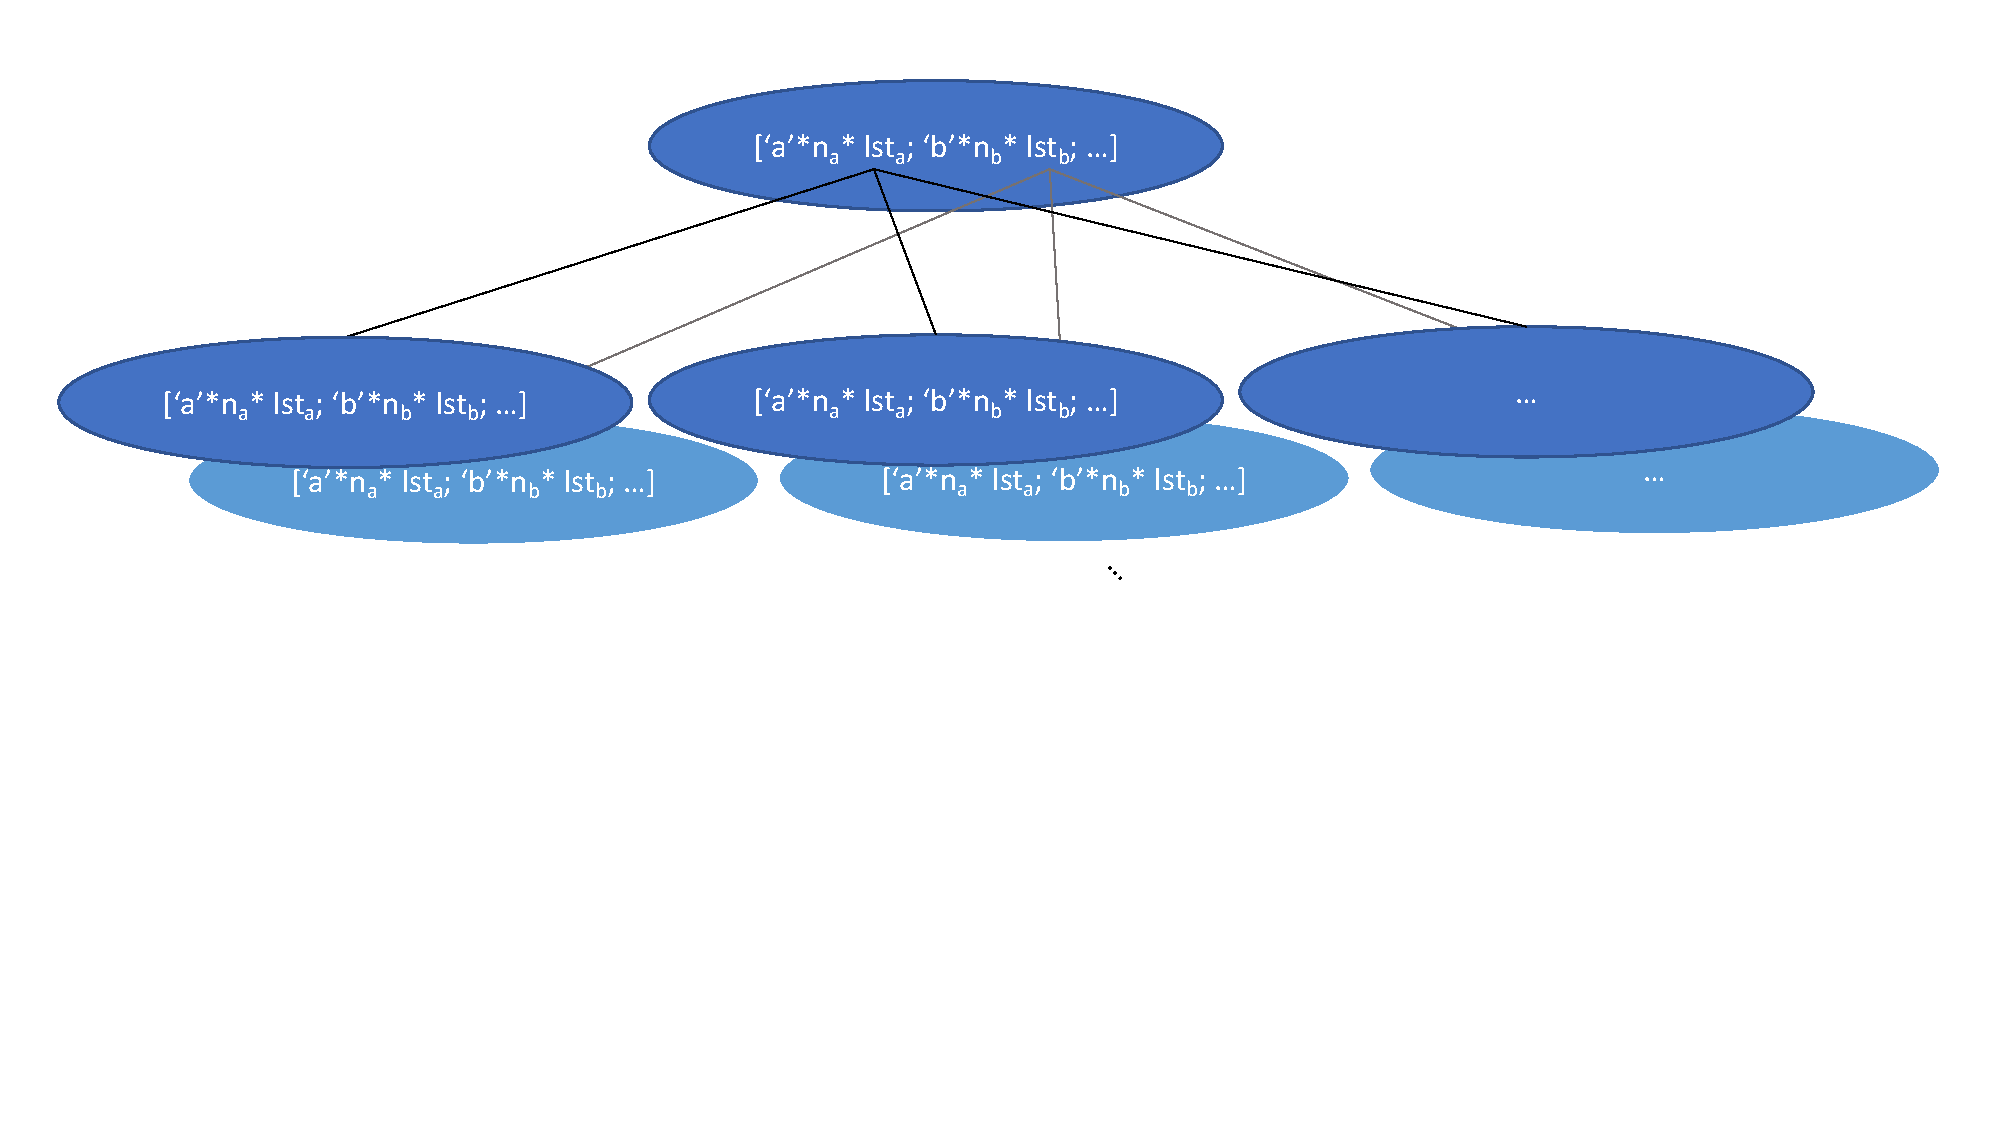
\includegraphics[width=\textwidth]{treeType}
  \caption{An illustration of a list of values of the type \lstinline{Tree}.}
  \label{fig:treeType}
\end{figure}
Words are to be represented as the sequence of characters from the
root til a node. The associated integer to each node counts the
occurrence of a word ending in that node. Thus, if the count is 0, then
no word with that endpoint has occurred. For example, a string with the
words ``a abc ba'' should result in the following tree,
\begin{quote}
  \mbox{\lstinline![Node ('a', 1, [Node ('b', 0, [Node ('c', 1, [])])]);!}\\
  \mbox{\hspace{0.5em}\lstinline!Node ('b', 0, [Node ('a', 1, [])])]!}
\end{quote}
Notice, the counts are zero for the combinations ``ab'' and ``b'',
which are words not observed in the string. The function must have the type:
\begin{quote}
  \mbox{\lstinline!wordHistogram : src:string -> Tree list!}
\end{quote}
Write a program which reads the text \lstinline[language=console]{littleClausAndBigClaus.txt}, discard all characters that are not in \lstinline{['a'..'z', 'A'..'Z',' ']}, convert all the remaining characters to lower case and calculate the occurrence of the remaining words as a \lstinline{Tree list} type.

 \item Write a white-box test of \lstinline{wordHistogram}, and add it to
your test file.

\item For a given value of a \lstinline!Tree! type, see
Exercise~\ref{wordHistogram}, write a function
\begin{quote}
  \mbox{\lstinline!randomWords : wHist:Tree list -> nWords:int -> string!}
\end{quote}
which generates a string with \lstinline!nWords! number of words
randomly selected to match the word distribution in
\lstinline!wHist!.

Use the function developed in Exercise~\ref{lowercase} and~\ref{wordHistogram}, and test
your function by generating a random string, whose words are
distributed as the converted characters in H.C.\ Andersen's fairy
tale, ``Little Claus and Big Claus''. Calculate the word histogram for
the random text, and compare this with \lstinline{wHist}.

\item The function \lstinline{randomWords} is a random function, and you are
to test its output by the histogram of the words in the string it
produces.

Extend your library with the function,
\begin{quote}
  \mbox{\lstinline!diffw : t1:Tree list -> t2:Tree list -> double!}
\end{quote}
which compares two word-histograms as the average sum of squared differences,
\begin{equation}
  \text{diffw}(t_1, t_2) = \frac{1}{M}\sum_{i=0}^{M-1}\left(t_1(i) - t_2(i)\right)^2
\end{equation}
where $t_1$ and $t_2$ are two word histograms, and $M$ is the total
number of different words observed in the two texts.

Extend your test file with a test of \lstinline{randomWords}
as follows:
\begin{enumerate}
\item Convert The Story using \lstinline{convertText} and calculate
  its word histogram.
\item Use this to generate a random text using \lstinline{randomWords} with
  $M$ words, where $M$ is the number of words in the converted The Story.
\item Calculate the distance between the word histograms of The Story
  and the random texts using \lstinline{diffw}.
\item Set the test as passed if the difference is below some threshold.
\end{enumerate}
You must choose a threshold in the above, and you must argue for your choice.

\item In terms of a Markov Chain, what order is \lstinline{randomWords}?
Suggest an extension of \lstinline{type Tree} to include first order
Markov Chains. Speculate on whether this principle can be used to
extend to n'th order mordels, and, in case, speculate on how the
storage requirements will grow as n grows.
\item Write a short report, which 
\begin{itemize}
\item is no larger than 5 pages;
\item contains a brief discussion on how your implementation works,
  and if there are any possible alternative implementations, and in that
  case, why you chose the one, you did;
\item includes output that demonstrates that your solutions work as intented.
\end{itemize}
%The report is to be handed in as a pdf document together with the single F\# source code as an fsx file.

\end{enumerate}

\end{document}

